\subsection{The Lattice of Subgroups of a Group}

\begin{exercise}[2.5.1]
    Let $H$ and $K$ be subgroups of $G$. Exhibit all possible sublattices which show only $G, 1, H, K$ and their joins and intersections. What distinguishes the different drawings?
\end{exercise}

\begin{sol}
    If $H$ and $K$ are distinct and neither is contained in the other, then the sublattice is a diamond shape. Otherwise, one of $H$ or $K$ is contained in the other, or they are equal, leading to a chain structure.
    \begin{center}
        \begin{tikzpicture}
            \node (G) at (0, 0) {$G$};
            \node (HK) at (0, -1) {$\gen{H, K}$};
            \node (H) at (-1, -2) {$H$};
            \node (K) at (1, -2) {$K$};
            \node (HnK) at (0, -3) {$H \cap K$};
            \node (1) at (0, -4) {$1$};

            \draw (G) -- (HK) -- (H) -- (HnK) -- (1);
            \draw (HK) -- (K) -- (HnK);

            \node (G2) at (4, 0) {$G$};
            \node (H2) at (4, -4/3) {$H$};
            \node (K2) at (4, -8/3) {$K$};
            \node (12) at (4, -4) {$1$};

            \draw (G2) -- (H2) -- (K2) -- (12);
        \end{tikzpicture}
    \end{center}
\end{sol}

\begin{exercise}[2.5.2]
    In each of (a) to (d) list all subgroups of $D_{16}$ that satisfy the given condition.
    \begin{subexercises}
        \item Subgroups that are contained in $\gen{sr^2, r^4}$
        \item Subgroups that are contained in $\gen{sr^7, r^4}$
        \item Subgroups that contain $\gen{r^4}$
        \item Subgroups that contain $\gen s$.
    \end{subexercises}
\end{exercise}

\begin{sol}
    Using the subgroup lattice of $D_{16}$, we find:
    \begin{subexercises}
        \item $\gen{sr^2, r^4}, \gen {sr^6}, \gen{sr^2}, \gen{r^4}, 1$.
        \item $\gen{sr^3, r^4}, \gen{r^4}, \gen{sr^3}, \gen{sr^7}, 1$.
        \item $\gen{r^4}, \gen{sr^2, r^4}, \gen{s, r^4}, \gen{r^2}, \gen{sr^3, r^4}, \gen{sr^5, r^4}, \gen{s, r^2}, \gen r, \gen{sr, r^2}, D_{16}$.
        \item $\gen s, \gen{s, r^4}, \gen{s, r^2}, D_{16}$. \qh
    \end{subexercises}
\end{sol}


\begin{exercise}[2.5.3]
    Show that the subgroup $\gen{s, r^2}$ of $D_8$ is isomorphic to $V_4$.
\end{exercise}

\begin{sol}
    Note that $\gen{s, r^2} = \set{1, s, r^2, sr^2}$. Consider the mapping $\phi : V_4 \to \gen{s, r^2}$ defined by
    \[
    	\phi(1) = 1, \quad \phi(a) = s, \quad \phi(b) = r^2, \quad \phi(c) = sr^2.
    \]
    To see that $\phi$ is a homomorphism, we can check a pair of non-identity elements, for example:
    \[
    	\phi(a)\phi(b) = s \cdot r^2 = sr^2 = \phi(c) = \phi(ab).
    \]
    Similar checks for the other pairs show that $\phi$ preserves the group operation. Since $\gen{s, r^2}$ has order 4 and $\phi$ is surjective, it follows that $\phi$ is also injective, and hence an isomorphism. Therefore, $\gen{s, r^2} \cong V_4$.
\end{sol}

\begin{exercise}[2.5.4]
    Use the given lattice to find all pairs of elements that generate $D_8$ (there are 12 pairs).
\end{exercise}

\begin{sol}
    Note that $D_8 = \gen{s, r}$. Moreover, $s \neq rs$, and $r \in \gen{s, rs}$ so that $\gen{s, rs} = D_8$. Since $r = r^3$, we also have $\gen{s, r^3} = D_8$. We may also replace the reflection $s$ with $sr^2$, since combinations of a reflection with an odd rotation and a reflection with an even rotation contain $r$ and thus generates $D_8$. It follows that the pairs of elements that generate $D_8$ are:
    \[
    	\gen{s, r}, \gen{s, r^3}, \gen{s, rs}, \gen{s, r^3s}, \gen{r^2s, r}, \gen{r^2s, r^3}, \gen{r^2s, rs}, \gen{r^2s, r^3s}, \gen{r, rs}, \gen{r^3, rs}, \gen{r, r^3s}, \gen{r^3, r^3s} \qh
    \]
\end{sol}

\begin{exercise}[2.5.5]
    Use the given lattice to find all elements $x \in D_{16}$ such that $D_{16} = \gen{x, s}$ (there are 8 such elements $x$).
\end{exercise}

\begin{sol}
    Note that $\gen r= \gen{r^3} = \gen{r^5} = \gen{r^7}$. We then pair each generator with an $s$ so that we obtain just the rotation to then generate $D_{16}$: $x = r, r^3, r^5, r^7, sr, sr^3, sr^5, sr^7$.
\end{sol}

\begin{exercise}[2.5.6]
    Use the given lattices to help find the centralizers of every element in the following groups:
    \begin{subexercises}
        \item $D_8$ \quad (b) $Q_8$ \quad (c) $S_3$ \quad (d) $D_{16}$.
    \end{subexercises}
\end{exercise}

\begin{solenum}
    \item To find $C_G(a)$ for some $a \in G$, we look for elements in $g \in G$ such that $g \notin \gen a$, but $ga = ag$, then look for the smallest subgroup containing both $\gen a$ and $g$.
    \begin{align*}
        C_{D_8}(1) & = D_8 & C_{D_8}(s) & = \gen{s, r^2} \\
        C_{D_8}(r) & = \gen r & C_{D_8}(rs) & = \gen{rs, r^2} \\
        C_{D_8}(r^2) & = D_8 & C_{D_8}(r^2s) & = \gen{s, r^2} \\
        C_{D_8}(r^3) & = \gen r & C_{D_8}(r^3s) & = \gen{sr, r^2}
    \end{align*}
    \item Note that $1, -1 \in Z(Q_8)$, while none of $i, j$, and $k$ commute with anything but themselves. Then:
    \begin{align*}
        C_{Q_8}(1) & = C_{Q_8}(-1) = Q_8 \\
        C_{Q_8}(i) & = C_{Q_8}(-i) = \gen i \\
        C_{Q_8}(j) & = C_{Q_8}(-j) = \gen j \\
        C_{Q_8}(k) & = C_{Q_8}(-k) = \gen k
    \end{align*}
    \item Note that no element of $S_3$ commutes with other elements, then $C_{S_3}(a) = \gen a$ for $a \in S_3 - \set 1$.
    \item Use similar reasoning as in part (a) to obtain the centralizers:
    \begin{align*}
        C_{D_{16}}(1) = C_{D_{16}}(r^4) & = D_{16} \\
        C_{D_{16}}(r^k) & = \gen r \text{ for all $k = 1, 2, 3, 5, ,6, $} \\
        C_{D_{16}}(s) = C_{D_{16}}(sr^4) & = \gen{s, r^4} \\
        C_{D_{16}}(sr) = C_{D_{16}}(sr^5) & = \gen{sr^5, r^4} \\
        C_{D_{16}}(sr^2) = C_{D_{16}}(sr^6) & = \gen{sr^2, r^4} \\
        C_{D_{16}}(sr^3) = C_{D_{16}}(sr^7) & = \gen{sr^3, r^4} \qh
    \end{align*}
\end{solenum}

\begin{exercise}[2.5.7]
    Find the center of $D_{16}$.
\end{exercise}

\begin{sol}
    $Z(D_{16}) = \set{1, r^4}$ by \exref{2.2.7}.
\end{sol}

\begin{exercise}[2.5.8]
    In each of the following groups find the normalizer of each subgroup:
    \begin{subexercises}
        \item $S_3$ \quad (b)~~$Q_8$.
    \end{subexercises}
\end{exercise}

\begin{solenum}
    \item From the subgroup lattice of $S_3$, each non-trivial subgroup is cyclic and maximal. Then $N_{S_3}(\gen\alpha) = \gen\alpha$ or $S_3$. For any 2-cycle $\alpha$, note that $\alpha\beta \neq \beta\alpha$ for any other 2-cycle $\beta$, hence $N_{S_3}(\gen\alpha) = \gen\alpha$. For the 3-cycle $\alpha = (1\ 2\ 3)$, any 2-cycle $\beta$ satisfies $\beta\alpha\beta\inv \in \gen\alpha$, so $N_{S_3}(\gen\alpha) = S_3$.
    \item Since $Z(Q_8) = \gen{-1}$, then $N_{Q_8}(\gen{-1}) = Q_8$. Similarly, $N_{Q_8}(\set 1) = Q_8$. For the subgroups of order 4, note that $ji(-j) = -i$ and $j(-i)(-j) = i$, so that $j \in N_{Q_8}(\gen i)$. Then $N_{Q_8}(\gen i) = Q_8$. By symmetry, the same holds for $\gen j$ and $\gen k$.
\end{solenum}


\begin{exercise}[2.5.9]
    Draw the lattices of subgroups of the following groups:
    \begin{subexercises}
        \item $\intmod[16]$ \quad (b) $\intmod[24]$ \quad (c) $\intmod[48]$.
    \end{subexercises}
\end{exercise}

\begin{sol}
    \phantom{x}
    \begin{center}
        \begin{tikzpicture}
            \node (g16) at (0, 6) {$\intmod[16]$};
            \node (2_16) at (0, 4.8) {$\gen 2$};
            \node (4_16) at (0, 3.6) {$\gen 4$};
            \node (8_16) at (0, 2.4) {$\gen 8$};
            \node (16_16) at (0, 1.2) {$\gen{16}$};

            \draw (g16) -- (2_16) -- (4_16) -- (8_16) -- (16_16);

            \node (g24) at (3, 6) {$\intmod[24]$};
            \node (3_24) at (2, 4.8) {$\gen 3$};
            \node (2_24) at (4, 4.8) {$\gen 2$};
            \node (6_24) at (3, 3.6) {$\gen 6$};
            \node (4_24) at (5, 3.6) {$\gen 4$};
            \node (12_24) at (4, 2.4) {$\gen{12}$};
            \node (8_24) at (6, 2.4) {$\gen 8$};
            \node (24_24) at (5, 1.2) {$\gen{24}$};

            \draw (g24) -- (3_24) -- (6_24) -- (12_24) -- (24_24);
            \draw (g24) -- (2_24) -- (4_24) -- (8_24) -- (24_24);
            \draw (6_24) -- (2_24);
            \draw (12_24) -- (4_24);

            \node (g48) at (8, 6) {$\intmod[48]$};
            \node (3_48) at (7, 4.8) {$\gen 3$};
            \node (2_48) at (9, 4.8) {$\gen 2$};
            \node (6_48) at (8, 3.6) {$\gen 6$};
            \node (4_48) at (10, 3.6) {$\gen 4$};
            \node (12_48) at (9, 2.4) {$\gen{12}$};
            \node (8_48) at (11, 2.4) {$\gen 8$};
            \node (24_48) at (10, 1.2) {$\gen{24}$};
            \node (16_48) at (12, 1.2) {$\gen{16}$};
            \node (48_48) at (11, 0) {$\gen{48}$};

            \draw (g48) -- (3_48) -- (6_48) -- (12_48) -- (24_48) -- (48_48);
            \draw (g48) -- (2_48) -- (4_48) -- (8_48) -- (16_48) -- (48_48);
            \draw (6_48) -- (2_48);
            \draw (12_48) -- (4_48);
            \draw (24_48) -- (8_48);
        \end{tikzpicture}
    \end{center}\vspace{-3ex}
\end{sol}

\begin{spex}[2.5.10]
    Classify groups of order 4 by proving that if $\abs G = 4$, then $G \cong Z_4$ or $G \cong V_4$.

    \hint{cf. \exref{1.1.36}.}
\end{spex}

\begin{sol}
    Let $G = \set{1, a, b, c}$.  If $G$ has an element of order 4, then $G \cong Z_4$ by Theorem 2.4.

    Suppose $G$ is not cyclic. Then every non-identity element has order 2 by Lagrange's Theorem. In particular, $a^2 = b^2 = c^2 = 1$. Note that $ab \neq 1$, since otherwise $b = a\inv = a$. Similarly, $ab \neq a$ and $ab \neq b$, so that $ab = c$. By similar reasoning, we have $bc = a$ and $ca = b$. This is precisely the definition of $V_4$, so that $G \cong V_4$.
\end{sol}


\begin{exercise} [2.5.11] 
    Consider the group of order 16 with the following presentation:
    \[
    	QD_{16} = \gen{\sigma, \tau \mid \sigma^8 = \tau^2 = 1, \sigma\tau = \tau\sigma^3}
    \]
    (called the \textbf{quasidihedral} or \textbf{semidihedral} group of order 16). This group has three subgroups of order 8: $\gen{\tau, \sigma^2} \cong D_8, \gen \sigma \cong Z_8$, and $\gen{\sigma^2, \sigma\tau} \cong Q_8$, and every proper subgroup is contained in one of these three subgroups. Fill in the missing subgroups in the lattice of all subgroups of the quasidihedral group, exhibiting each subgroup with at most two generators.
    \begin{center}
        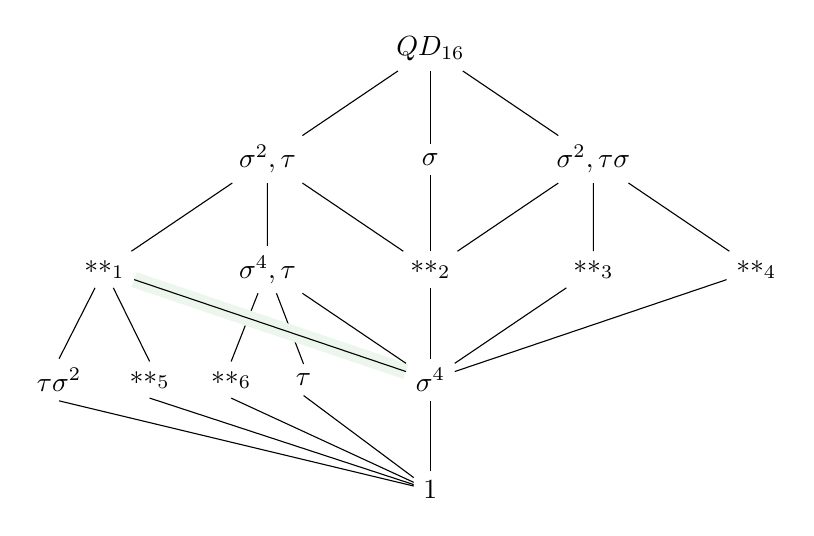
\begin{tikzpicture}[xscale=1.15, yscale=1.4]
            \node (G) at (0, 0) {$QD_{16}$};

            \node (s2t) at (-1.8, -1) {$\gen{\sigma^2, \tau}$};
            \node (s) at (0, -1) {$\gen \sigma$};
            \node (s2ts) at (1.8, -1) {$\gen{\sigma^2, \tau\sigma}$};

            \node (u1) at (-3.6, -2) {$\gen{**}_1$};
            \node (s4t) at (-1.8, -2) {$\gen{\sigma^4, \tau}$};
            \node (u2) at (0, -2) {$\gen{**}_2$};
            \node (u3) at (1.8, -2) {$\gen{**}_3$};
            \node (u4) at (3.6, -2){$\gen{**}_4$};

            \node (ts2) at (-4.1, -3) {$\gen{\tau\sigma^2}$};
            \node (u5) at (-3.1, -3) {$\gen{**}_5$};
            \node (u6) at (-2.2, -3) {$\gen{**}_6$};
            \node (t) at (-1.4, -3){$\gen \tau$};
            \node (s4) at (0, -3) {$\gen{\sigma^4}$};

            \node (1) at (0, -4) {1};

            \draw (1) -- (ts2.south);
            \draw (ts2.north) -- (u1) -- (s2t) -- (G);
            \draw (1) -- (u5.south);
            \draw (u5.north) -- (u1);
            \draw (1) -- (u6.south);
            \draw (u6.north) -- (s4t) -- (s2t);
            \draw (1) -- (t.south);
            \draw (t.north) -- (s4t);
            \draw (1) -- (s4) -- (u2) -- (s) -- (G);
            \draw [preaction={draw, line width=2mm, color=Green!7!White}] (s4) -- (u1);
            \draw (s4) -- (s4t);
            \draw (s4) -- (u3) -- (s2ts) -- (G);
            \draw (s4) -- (u4) -- (s2ts);
            \draw (u2) -- (s2t);
            \draw (u2) -- (s2ts);
        \end{tikzpicture}
    \end{center}
\end{exercise}

\begin{sol}
    The above has had subscripts added to distinguish the unknown subgroups. It is clear that $\gen{**}_2$ must be $\gen{\sigma^2}$ since it is the only subgroup contained in both $\gen \sigma$ and $\gen{\sigma^2, \tau}$. To find the other subgroups, we calculate the cyclic subgroups of the form $\gen{\tau\sigma^k}$:
    \begin{align*}
        \gen{\tau\sigma} & = \set{1, \tau\sigma, \sigma^4, \tau\sigma^5} & \gen{\tau\sigma^3} & = \set{1, \tau\sigma^3, \sigma^4, \tau\sigma^7} \\
        \gen{\tau\sigma^4} & = \set{1, \tau\sigma^4} & \gen{\tau\sigma^6} & = \set{1, \tau\sigma^6}
    \end{align*}
    It becomes clear that 6 must be $\gen{\tau\sigma^4}$, since the subgroup above contains both $\tau$ and $\sigma^4$. 3 and 4 must be $\gen{\tau\sigma}$ and $\gen{\tau\sigma^3}$ respectively, since $\gen{\sigma^2, \tau\sigma}$ both contain $\tau\sigma$ and $\sigma^2$ which multiply to $\tau\sigma^3$. Certainly, 1 cannot be $\gen{\tau\sigma^6}$ as it does not contain $\gen{\tau\sigma^2}$, so it must be 5. Then 1 must be $\gen{\tau\sigma^2, \sigma^4}$ as it contains both subgroups. Hence, the completed diagram is
    \begin{center}
        \begin{tikzpicture}[xscale=1.15, yscale=1.4]
            \node (G) at (0, 0) {$QD_{16}$};

            \node (s2t) at (-1.8, -1) {$\gen{\sigma^2, \tau}$};
            \node (s) at (0, -1) {$\gen \sigma$};
            \node (s2ts) at (1.8, -1) {$\gen{\sigma^2, \tau\sigma}$};

            \node (u1) at (-3.6, -2) {$\gen{\tau\sigma^2, \sigma^4}$};
            \node (s4t) at (-1.8, -2) {$\gen{\sigma^4, \tau}$};
            \node (u2) at (0, -2) {$\gen{\sigma^2}$};
            \node (u3) at (1.8, -2) {$\gen{\tau\sigma}$};
            \node (u4) at (3.6, -2){$\gen{\tau\sigma^3}$};

            \node (ts2) at (-4.1, -3) {$\gen{\tau\sigma^2}$};
            \node (u5) at (-3.1, -3) {$\gen{\tau\sigma^6}$};
            \node (u6) at (-2.2, -3) {$\gen{\tau\sigma^4}$};
            \node (t) at (-1.4, -3){$\gen \tau$};
            \node (s4) at (0, -3) {$\gen{\sigma^4}$};

            \node (1) at (0, -4) {1};

            \draw (1) -- (ts2.south);
            \draw (ts2.north) -- (u1) -- (s2t) -- (G);
            \draw (1) -- (u5.south);
            \draw (u5.north) -- (u1);
            \draw (1) -- (u6.south);
            \draw (u6.north) -- (s4t) -- (s2t);
            \draw (1) -- (t.south);
            \draw (t.north) -- (s4t);
            \draw (1) -- (s4) -- (u2) -- (s) -- (G);
            \draw [preaction={draw, line width=2mm, pagecolor!50}] (s4) -- (u1);
            \draw (s4) -- (s4t);
            \draw (s4) -- (u3) -- (s2ts) -- (G);
            \draw (s4) -- (u4) -- (s2ts);
            \draw (u2) -- (s2t);
            \draw (u2) -- (s2ts);
        \end{tikzpicture}
    \end{center}
\end{sol}

\begin{exercise} [2.5.12] 
    The group $A = Z_2 \times Z_4 = \gen{a, b \mid a^2 = b^4 = 1, ab = ba}$ has order 8 and has three subgroups of order 4: $\gen{a, b^2} \cong V_4, \gen b \cong Z_4$, and $\gen{ab} \cong Z_4$ and every proper subgroup is contained in one of these three. Draw the lattice of all subgroups of $A$, giving each subgroup in terms of at most two generators.
\end{exercise}

\begin{sol}
    Since $A$ is the direct product of two Abelian groups, it itself is Abelian, and we may write:
    \[
    	A = \set{1, b, b^2, b^3, a, ab, ab^2, ab^3}
    \]
    Using the isomorphisms given, we construct the lattice.
    \begin{center}
        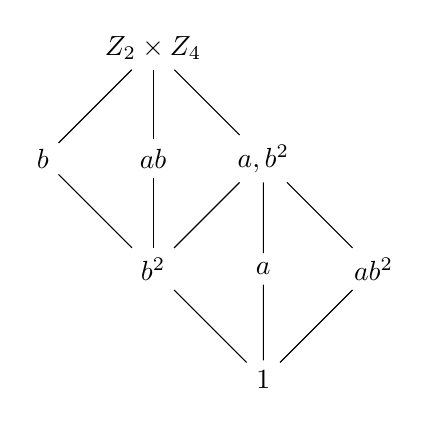
\begin{tikzpicture}[scale=1.4]
            \node (A) at (0, 0) {$Z_2 \times Z_4$};
            
            \node (b) at (-1, -1) {$\gen b$};
            \node (ab) at (0, -1) {$\gen{ab}$};
            \node (a b2) at (1, -1) {$\gen{a, b^2}$};

            \node (b2) at (0, -2) {$\gen{b^2}$};
            \node (a) at (1, -2) {$\gen a$};
            \node (ab2) at (2, -2) {$\gen{ab^2}$};

            \node (1) at (1, -3) {1};

            \draw (1) -- (b2) -- (b) -- (A);
            \draw (1) -- (a) -- (a b2) -- (A);
            \draw (b2) -- (ab) -- (A);
            \draw (b2) -- (a b2);
            \draw (1) -- (ab2) -- (a b2);
        \end{tikzpicture}
    \end{center}
\end{sol}

\begin{exercise} [2.5.13]
    The group $G = Z_2 \times Z_8 = \gen{x, y \mid x^2 = y^8 = 1, xy = yx}$ has order 16 and has three subgroups of order 8: $\gen{x, y^2} \cong Z_2 \times Z_4, \gen y \cong Z_8$, and $\gen{xy} \cong Z_8$, and every proper subgroup is contained in one of those three. Draw the lattice of all subgroups of $G$, giving each subgroups in terms of at most two generators (cf. \exref{2.5.12}).
\end{exercise}

\begin{sol}
    Put $x = a$ and $y^2 = b$, where $\gen{a, b}$ is \exref{2.5.12}. Then $G$ contains a copy of $Z_2 \times Z_4$, with the necessary appending of $\gen y$ and $\gen{xy}$ to the lattice:
    \begin{center}
        \begin{tikzpicture}[scale=1.4]
            \node (G) at (0, 0) {$G$};

            \node (y) at (-1, -1) {$\gen y$};
            \node (xy) at (0, -1) {$\gen{xy}$};
            \node (x y2) at (1, -1) {$\gen{x, y^2}$};

            \node (y2) at (0, -2) {$\gen{y^2}$};
            \node (xy2) at (1, -2) {$\gen{xy^2}$};
            \node (x y4) at (2, -2) {$\gen{x, y^4}$};

            \node (y4) at (1, -3) {$\gen{y^4}$};
            \node (x) at (2, -3) {$\gen x$};
            \node (xy4) at (3, -3) {$\gen{xy^4}$};

            \node (1) at (2, -4) {1};

            \draw (1) -- (y4) -- (y2) -- (y) -- (G);
            \draw (1) -- (xy4) -- (x y4) -- (x y2) -- (G);
            \draw (1) -- (x) -- (x y4);
            \draw (y4) -- (xy2) -- (x y2);
            \draw (y2) -- (xy) -- (G);
            \draw (y4) -- (x y4);
            \draw (y2) -- (x y2);
        \end{tikzpicture}
    \end{center}\vspace{-3ex}
\end{sol}

\begin{spex}[2.5.14] 
    Let $M$ be the \textbf{modular group} of order 16 with the following presentation:
    \[
    	\gen{u, v \mid u^2 = v^8 = 1, vu = uv^5}.
    \]
    It has three subgroups of order 8: $\gen{u, v^2}, \gen v$, and $\gen{uv}$, and every proper subgroup is contained in one of those three. Prove that $\gen{u, v^2} \cong Z_2 \times Z_4, \gen v \cong Z_8$, and $\gen{uv} \cong Z_8$. Show that the lattice of subgroups of $M$ is the same as the lattice of subgroups of $Z_2 \times Z_8$ (cf. \exref{2.5.13}) but that these two groups are not isomorphic.
\end{spex}

\begin{sol}
    Since $\abs v = \abs{uv} = 8$, then $\gen v \cong \gen{uv} \cong Z_8$. One can apply the second relation to obtain $v^2u = uv^2$, hence we deduce that $\gen{u, v^2}$ is Abelian. We may write
    \[
    	\gen{u, v^2} = \set{1, v^2, v^4, v^6, u, uv^2, uv^4, uv^6}
    \]
    From the enumeration of $\gen{u, v^2}$, we have the map $\phi : Z_2 \times Z_4 \to \gen{u, v^2}$ defined by
    \[
    	\phi(a) = u, \quad \phi(b) = v^2.
    \]
    This extends to a homomorphism. Moreover, $|\gen{u, v^2}| = |Z_2 \times Z_4| = 8$. Since $\phi$ sends distinct elements of $Z_2 \times Z_4$ to distinct elements of $\gen{u, v^2}$, it is injective. Being a homomorphism between two groups of the same finite order, it is also surjective, hence an isomorphism. We have the following lattice for $M$:
    \begin{center}
        \begin{tikzpicture}[scale = 1.3]
            \node (G) at (0, 0) {$G$};

            \node (y) at (-1, -1) {$\gen v$};
            \node (xy) at (0, -1) {$\gen{uv}$};
            \node (x y2) at (1, -1) {$\gen{u, v^2}$};

            \node (y2) at (0, -2) {$\gen{v^2}$};
            \node (xy2) at (1, -2) {$\gen{uv^2}$};
            \node (x y4) at (2, -2) {$\gen{u, v^4}$};

            \node (y4) at (1, -3) {$\gen{v^4}$};
            \node (x) at (2, -3) {$\gen u$};
            \node (xy4) at (3, -3) {$\gen{uv^4}$};

            \node (1) at (2, -4) {1};

            \draw (1) -- (y4) -- (y2) -- (y) -- (G);
            \draw (1) -- (xy4) -- (x y4) -- (x y2) -- (G);
            \draw (1) -- (x) -- (x y4);
            \draw (y4) -- (xy2) -- (x y2);
            \draw (y2) -- (xy) -- (G);
            \draw (y4) -- (x y4);
            \draw (y2) -- (x y2);
        \end{tikzpicture}
    \end{center}
    Since $vu = uv^5 \neq uv$, $M$ is not Abelian, and therefore cannot be isomorphic to $Z_2 \times Z_8$.
\end{sol}


\begin{exercise}[2.5.15]
    Describe the isomorphism type of each of the three subgroups of $D_{16}$ of order 8.
\end{exercise}

\begin{sol}
    From $\abs r = 8$, we deduce $\gen r \cong Z_8$. The remaining subgroups $\gen{s, r^2}$ and $\gen{sr, r^2}$ can be shown to be isomorphic to $D_8$ as follows:
    \begin{itemize}
        \item For the subgroup $\gen{s, r^2}$, observe that $(r^2)^4 = s^2 = 1$, and $sr^2 = r^6s = (r^2)\inv s$. Use $r^2$ in place of $r$ and $s$ in place of $s$ to see that the relations match those of $D_8$.
        \item For the subgroup $\gen{sr, r^2}$, observe that $(r^2)^4 = (sr)^2 = 1$, and \[
 	(sr)r^2 = sr^3 = r^5s = r^6r^7s = (r^2)\inv(sr).
 \]
        Use $r^2$ in place of $r$ and $sr$ in place of $s$ to see that the relations match those of $D_8$. \qh
    \end{itemize}
\end{sol}

\begin{exercise}[2.5.16]
    Use the lattice of subgroups of the quasidihedral of order 16 to show that every element of order 2 is contained in the proper subgroup $\gen{\tau, \sigma^2}$ (cf. \exref{2.5.11}).
\end{exercise}

\begin{sol}
    Every element of order 2 generates a cyclic subgroup of order 2. Using the lattice, $\gen{\tau, \sigma^2}$ properly contains all cyclic subgroups, except $\gen{\tau\sigma}$ and $\gen{\tau\sigma^3}$, both of which are order 4. Then $\gen{\tau, \sigma^2}$ contains all cyclic subgroups of order 2, hence contain all elements of order 2.
\end{sol}

\begin{exercise}[2.5.17]
    Use the lattice of subgroups of the modular group $M$ of order 16 to show that the set $\set{x \in M \mid x^2 = 1}$ is a subgroup of $M$ isomorphic to the Klein 4-group (cf. \exref{2.5.14}).
\end{exercise}

\begin{sol}
    Using the lattice in Exercise 14, we see that we have 3 candidates to be isomorphic to $V_4$, namely $\gen{v^2}, \gen{uv^2},$ and $\gen{u, v^4}$. The first and second subgroups are cyclic, while $\gen{u, v^4} = \set{1, u, v^4, uv^4}$. Since it is not generated by one element, each of these elements are of order 2, and $v^4u = v^3uv^5 = \cdots = uv^{20} = uv^4$ so that it is Abelian, then $\gen{u, v^4} \cong V_4$.
\end{sol}

\begin{exercise}[2.5.18]
    Use the lattice to help find the centralizer of every element of $QD_{16}$ (cf. \exref{2.5.11}).
\end{exercise}

\begin{sol}
    Note that $\sigma^4\tau = \sigma^3\tau\sigma^3 = \cdots = \tau\sigma^{12} = \tau\sigma^4$ so that $\sigma^4 \in Z(QD_{16})$ as $\sigma^4$ already commutes with powers of $\sigma$. Moreover, any power of $\sigma$ does not commute with $\tau$ except for $\sigma^4$. The elements $\tau\sigma$ and $\tau\sigma^3$ do not commute with $\sigma^2$ as $(\tau\sigma)\sigma^2 = \tau\sigma^3 = \sigma\tau \neq \sigma^2(\tau\sigma) = \tau\sigma^2$, and $(\tau\sigma^3)\sigma^2 = \sigma^7\tau \neq \sigma^3\tau = \sigma^2(\tau\sigma^3)$. Next, $(\tau\sigma^2)\sigma^2 = \tau\sigma^4 \neq \tau = \sigma^2(\tau\sigma^2)$ so that $\sigma^2$ does not commute with $\tau\sigma^2$. Moreover, $(\tau\sigma^6)(\tau\sigma^2) = \tau\sigma^2\sigma^4\tau\sigma^2 = (\tau\sigma^2)(\tau\sigma^6)$ so that $\tau\sigma^2$ commutes with $\tau\sigma^6$, but $\sigma^2\tau\sigma^6 = \tau\sigma^4 \neq \tau = (\tau\sigma^6)\sigma^2$ so $\sigma^2$ does not commute with $\tau\sigma^6$. Lastly, $\sigma^2(\tau\sigma^4) = \tau\sigma^2 \neq (\tau\sigma^4)\sigma^2$, and $\sigma^2\tau = \tau\sigma^6 \neq \tau\sigma^2$ so that $\sigma^2$ does not commute with $\tau\sigma^4$ nor with $\tau$. It follows that the centralizers of the elements of $QD_{16}$ are
    \begin{align*}
        C_{QD_{16}}(1) = C_{QD_{16}}(\sigma^4) & = QD_{16} \\
        C_{QD_{16}}(\gen{\sigma^k}) & = \gen\sigma \text{ for $k = 1, 2, 3, 5, 6, 7$} \\
        C_{QD_{16}}(\gen{\tau\sigma}) = C_{QD_{16}}(\gen{\tau\sigma^5}) & = \gen{\tau\sigma} \\
        C_{QD_{16}}(\gen{\tau\sigma^3}) = C_{QD_{16}}(\gen{\tau\sigma^7}) & = \gen{\tau\sigma^3} \\
        C_{QD_{16}}(\gen\tau) = C_{QD_{16}}(\gen{\tau\sigma^4}) & = \gen{\sigma^4, \tau} \\
        C_{QD_{16}}(\gen{\tau\sigma^2}) = C_{QD_{16}}(\gen{\tau\sigma^6}) & = \gen{\tau\sigma^2, \sigma^4}
    \end{align*}
\end{sol}

\begin{exercise}[2.5.19]
    Use the lattice to help find $N_{D_{16}}(\gen{s, r^4})$.
\end{exercise}

\begin{sol}
    Based on the placement of $\gen{s, r^4}$, its normalizer may be itself, $\gen{s, r^2}$, or $D_{16}$. Note that $\gen{s, r^4} = \set{1, s, r^4, sr^4}$, and taking $r^2$ and $(r^2)\inv = r^6$, we have
    \[
    	r^2\gen{s, r^4}r^6 = \set{1, sr^4, r^4, s} = \gen{s, r^4}
    \]
    so that $r^2 \in N_{D_{16}}(\gen{s, r^4})$, and $\gen{s, r^2} \leq N_{D_{16}}(\gen{s, r^4})$. Since $rsr\inv = r^2s \neq r$, then $r \notin N_{D_{16}}(\gen{s, r^4})$ so that $N_{D_{16}}(\gen{s, r^4}) = \gen{s, r^2}$.
\end{sol}

\begin{exercise}[2.5.20]
    Use the lattice of subgroups of $QD_{16}$ (cf. \exref{2.5.11}) to help find the normalizers
    \begin{subexercises}
        \item $N_{QD_{16}}(\gen{\tau\sigma})$ \quad (b)~~$N_{QD_{16}}(\gen{\tau, \sigma^4})$.
    \end{subexercises}
\end{exercise}

\begin{solenum}
    \item Note that $\gen{\tau\sigma} = \set{1, \tau\sigma, \sigma^4, \tau\sigma^5}$. Moreover, $(\sigma^2)\inv = \sigma^6$ so that
    \[
    	\sigma^2\gen{\tau\sigma}\sigma^6 = \set{1, \tau\sigma^4, \sigma^4, \tau\sigma} = \gen{\tau\sigma}
    \]
    and $\sigma(\tau\sigma)\sigma^7 = \tau\sigma^3 \neq \tau\sigma$ so that $\sigma \notin N_{QD_{16}}(\gen{\tau\sigma})$. Then $N_{QD_{16}}(\gen{\tau\sigma}) = \gen{\sigma^2, \tau\sigma}$.
    \item $\gen{\tau, \sigma^4} = \set{1, \tau, \sigma^4, \tau\sigma^4}$, and 
    \[
    	\sigma^2\gen{\tau, \sigma^4}\sigma^6 = \set{1, \tau\sigma^4, \sigma^4, \tau}
    \]
    while $\sigma\tau\sigma^7 = \tau\sigma^2 \neq \tau$ so that $\sigma \notin N_{QD_{16}}(\gen{\tau, \sigma^4})$. Then $N_{QD_{16}}(\gen{\tau, \sigma^4}) = \gen{\sigma^2, \tau}$.
\end{solenum}